\documentclass{article}



\usepackage{fullpage}
\usepackage{nopageno}
\usepackage{amsmath}
\usepackage{amsfonts}
\usepackage{graphicx}
\usepackage{framed}
\usepackage{xcolor}

\definecolor{dark_red}{rgb}{0.5,0.0,0.0}
\definecolor{dark_green}{rgb}{0.0,0.5,0.0}
\definecolor{dark_blue}{rgb}{0.0,0.0,0.5}

\newcommand{\dr}[1]{\textcolor{dark_red}{#1}}
\newcommand{\dg}[1]{\textcolor{dark_green}{#1}}
\newcommand{\db}[1]{\textcolor{dark_blue}{#1}}


\begin{document}

\section*{Interval Notation}

An {\bf interval} is a continuous set of real numbers between two endpoints. Consider an interval that is bounded by real numbers \(a\) and \(b\), where \(a\) is the lower bound, and \(b\) is the upper bound (\(a < b\)). The interval is denoted by \((a, b)\), \((a, b]\), \([a, b)\), and \([a, b]\) depending on whether the endpoints, \(a\) and \(b\), are included. A round parenthesis excludes the bound, while a square parenthesis includes the bound. The formal definition of the various interval types are given below. On the left, the various intervals are defined, while on the right, a depiction of these intervals is shown on the real number line. When drawing an interval on the real number line, the endpoints are marked with circles. An open circle excludes an endpoint, while a closed circle includes an endpoint. 

\begin{tabular}{cc}
\parbox{0.5\textwidth}{
\begin{itemize}
\item \((a, b) = \{x \in \mathbb{R} | a < x < b\}\) is the interval that contains all real numbers between \(a\) and \(b\), and {\bf excludes} the endpoints \(a\) and \(b\).
\item \((a, b] = \{x \in \mathbb{R} | a < x \leq b\}\) is the interval that contains all real numbers between \(a\) and \(b\), and {\bf excludes} \(a\), while {\bf includes} \(b\).
\item \([a, b) = \{x \in \mathbb{R} | a \leq x < b\}\) is the interval that contains all real numbers between \(a\) and \(b\), and {\bf includes} \(a\), while {\bf excludes} \(b\).
\item \([a, b] = \{x \in \mathbb{R} | a \leq x \leq b\}\) is the interval that contains all real numbers between \(a\) and \(b\), and {\bf includes} the endpoints \(a\) and \(b\).
\end{itemize}
} & \parbox{0.4\textwidth}{
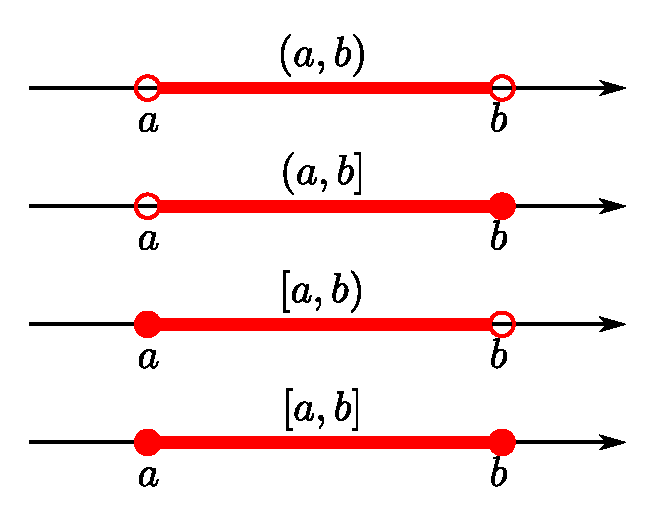
\includegraphics[width = 0.4\textwidth]{intervals}
}
\end{tabular}


\subsection*{Unions}

The {\bf union} of two sets \(A\) and \(B\) is a set that contains all elements that appear in at least one of the sets.

\[A \cup B = \{x | (x \in A) \vee (x \in B)\}\]
(recall that the symbol \(\vee\) means ``OR")

In the examples below, the lower two lines, the red and green lines, depict sets \(A\) and \(B\) respectively. The upper blue line depicts \(A \cup B\).

\textbf{Examples:}
\begin{itemize}
%%%%%%%%%%% 1
\item 
\[(-2, 3) \cup [4, 5)\]
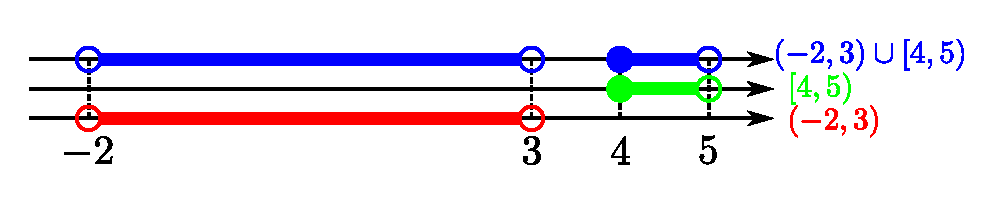
\includegraphics[scale = 0.9]{union_example_1}
%%%%%%%%%%% 2
\item 
\[(-2, 3) \cup [2, 5) = (-2, 5)\]
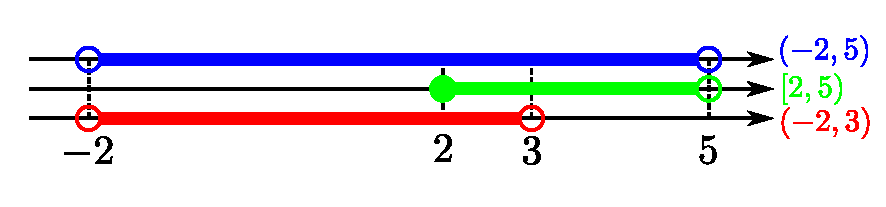
\includegraphics[scale = 0.9]{union_example_2}
%%%%%%%%%%% 3
\item
\[(-4, 2] \cup [-4, 0) = [-4, 2]\]
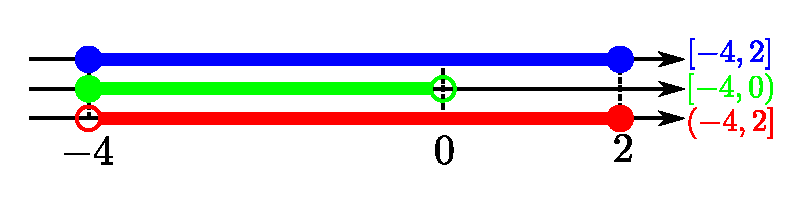
\includegraphics[scale = 0.9]{union_example_3}
%%%%%%%%%%% 4
\item 
\[[1, 2) \cup (2, 3]\]

\includegraphics[scale = 0.9]{union_example_4}
%%%%%%%%%%% 5
\item 
\[[1, 2) \cup [2, 3] = [1, 3]\]

\includegraphics[scale = 0.9]{union_example_5}
%%%%%%%%%%% 6
\item 
\[(0, 6) \cup \{6\} = (0, 6]\]

\includegraphics[scale = 0.9]{union_example_6}
\end{itemize}


\subsection*{Intersections}

The {\bf intersection} of two sets \(A\) and \(B\) is a set that contains all elements that appear in both of the sets.

\[A \cap B = \{x | (x \in A) \wedge (x \in B)\}\]
(recall that the symbol \(\wedge\) means ``AND")

In the examples below, the lower two lines, the red and green lines, depict sets \(A\) and \(B\) respectively. The upper blue line depicts \(A \cap B\).

\textbf{Examples:}
\begin{itemize}
%%%%%%%%%%% 1
\item 
\[(-\infty, 3] \cap [4, 5] = \emptyset\]
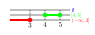
\includegraphics[scale = 0.9]{intersection_example_1}
%%%%%%%%%%% 2
\item 
\[[1, 3] \cap (2, +\infty) = (2, 3]\]
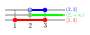
\includegraphics[scale = 0.9]{intersection_example_2}
%%%%%%%%%%% 3
\item 
\[(-4, -2] \cap [-4, -2) = (-4, -2)\]
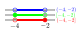
\includegraphics[scale = 0.9]{intersection_example_3}
%%%%%%%%%%% 4
\item 
\[(-3, 4] \cap [-1, 2) = [-1, 2)\]
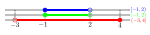
\includegraphics[scale = 0.9]{intersection_example_4}
%%%%%%%%%%% 4
\item 
\[[3, +\infty) \cap (-\infty, 5) = [3, 5)\]
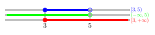
\includegraphics[scale = 0.9]{intersection_example_5}
\end{itemize}




\section*{Solving Inequalities}

Solving inequalities refers to taking statements of the form 
\begin{itemize}
\item \(f(x) \leq g(x)\)
\item \(f(x) < g(x)\)
\item \(f(x) \geq g(x)\)
\item \(f(x) > g(x)\)
\item \(f(x) \neq g(x)\) 
\end{itemize}
and finding the interval (set) of values for variable \(x\) that satisfy the given inequalities.


\subsection*{Revisiting equations} 

Given an equation \(f(x) = g(x)\), the truth of this equation is preserved if the same function \(h(X)\) is applied to both sides:
\[f(x) = g(x) \implies h(f(x)) = h(g(x))\]
This statement means that if \(f(x) = g(x)\) is true, then \(h(f(x)) = h(g(x))\) is also true.

~

Also, if the function \(h(X)\) is one-to-one, then converting \(f(x) = g(x)\) to \(h(f(x)) = h(g(x))\) results in no loss of information. As a reminder, function \(h(X)\) is one-to-one when no two different values of \(X\) give the same value of \(h(X)\):
\[\forall X_1, X_2 : X_1 \neq X_2 \implies h(X_1) \neq h(X_2)\]
The above statement reads as follows: For every pair of values \(X_1\) and \(X_2\), if \(X_1\) and \(X_2\) are not equal, then \(h(X_1)\) and \(h(X_2)\) are not equal.

Consider, for example, \(h(X) = X^2\). This function \(h(X) = X^2\) is {\bf not} one-to-one. Consider the equation \(x + 2 = 3\). This equation only allows \(x = 1\). Applying \(h(X)\) to both sides gives \((x + 2)^2 = 9\). The equation \((x + 2)^2 = 9\) allows for \(x = -5\) as well as \(x = 1\), and this means that \((x + 2)^2 = 9\) entails {\bf less} information than \(x + 2 = 3\). This information loss does not occur if \(h(X)\) is one-to-one, and hence if \(h(X)\) is one-to-one,
\[f(x) = g(x) \iff h(f(x)) = h(g(x))\]
This statement means that if \(f(x) = g(x)\) is true, then \(h(f(x)) = h(g(x))\) is also true {\bf and vice-versa}. Equations \(f(x) = g(x)\) and \(h(f(x)) = h(g(x))\) are therefore {\bf equivalent}.


\subsection*{Using inequalities}

Given the inequality \(f(x) \leq g(x)\), this inequality is conserved and retains all information if a {\bf strictly monotone increasing} function \(h(X)\) is applied to both sides. \\
\begin{tabular}{cc}
\parbox{0.5\textwidth}{
A function \(h(X)\) is {\bf strictly monotone increasing} when \(h(X)\) only increases when \(X\) increases. Moreover, \(h(X)\) does not loiter at any value.
\[\forall X_1, X_2 : X_1 < X_2 \implies h(X_1) < h(X_2)\]
The above statement reads as follows: For every pair of values \(X_1\) and \(X_2\), if \(X_1 < X_2\), then \(h(X_1) < h(X_2)\). \\
In the image of the right, the dark red curve is the graph of a strictly monotone increasing function \(h(X)\). The light green curve and the light blue curves are graphs of functions that are not strictly monotone increasing. The light green curve loiters at a value for multiple input values, while the light blue curve decreases for a certain range of input values. 
} & \parbox{0.5\textwidth}{
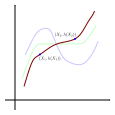
\includegraphics[width = 0.5\textwidth]{strictly_monotone_functions}
}
\end{tabular}
Similar to being strictly monotone increasing, a function \(h(X)\) is {\bf strictly monotone decreasing} if \(h(X)\) only decreases when \(X\) increases. Moreover, \(h(X)\) does not loiter at any value:
\[\forall X_1, X_2 : X_1 < X_2 \implies h(X_1) > h(X_2)\]

\vspace{5mm}

When \(h(X)\) is strictly monotone increasing, applying \(h(X)\) to both sides of the inequality \(f(x) \leq g(x)\) preserves not only the truth of the inequality, but also all information:
\[f(x) \leq g(x) \iff h(f(x)) \leq h(g(x))\]
The addition or subtraction of any value is monotone increasing. If \(c\) is any real number or expression, then 
\[f(x) \leq g(x) \iff f(x) + c \leq g(x) + c\]
The multiplication or division by any strictly positive value is monotone increasing. If \(k\) is any strictly positive (\(k > 0\)) real number or expression, then 
\[f(x) \leq g(x) \iff k \cdot f(x) \leq k \cdot g(x)\]  

\vspace{5mm}

When \(h(X)\) is strictly monotone decreasing, applying \(h(X)\) to both sides of the inequality \(f(x) \leq g(x)\) \emph{reverses} the inequality, and preserves all information:
\[f(x) \leq g(x) \iff h(f(x)) \geq h(g(x))\]
It is important to note that multiplication or division by a negative number is strictly monotone decreasing. If \(k\) is any strictly negative (\(k < 0\)) real number or expression, then
\[f(x) \leq g(x) \iff k \cdot f(x) \geq k \cdot g(x)\]

\vspace{5mm}

These same principles hold even if \(\leq\) is replaced with the stricter version \(<\).

Using these tools, inequalities can be manipulated until the set of values of \(x\) that satisfy the inequality becomes obvious:



\textbf{Example 1:}

Start with:
\[\frac{x + 2}{3} \geq 2\]
Multiplying both sides by \(3\) gives:
\[x + 2 \geq 6\]
Subtracting \(2\) from both sides gives:
\[x \geq 4\]
From this inequality, the set of values of \(x\) that satisfy this inequality, and hence the first inequality is:
\[[4, +\infty)\]

\vspace{5mm}



\textbf{Example 2:}

Start with:
\[x < 3x - 2\]
Subtracting \(3x\) from both sides gives: 
\[-2x < -2\]
Dividing both sides by \(-2\) gives:
\[x > 1\]
the inequality is reversed because multiplication or division by a negative number is strictly monotone decreasing. \\
From this inequality, the set of values of \(x\) that satisfy this inequality, and hence the first inequality is:
\[(1, +\infty)\]

\vspace{5mm}



\textbf{Example 3:}

Start with:
\[-6x + 10 \geq 52\]
Subtracting \(10\) from both sides gives:
\[-6x \geq 42\]
Dividing both sides by \(-6\) gives:
\[x \leq -7\]
From this inequality, the set of values of \(x\) that satisfy this inequality, and hence the first inequality is:
\[(-\infty, -7]\]

\vspace{5mm}



\textbf{Example 4:}

Start with the two inequalities: 
\[(2 - 3x < 8) \wedge (2x \leq 24 - 2x)\]
(recall that the symbol \(\wedge\) means ``AND")

Solving the first inequality, \(2 - 3x < 8\), subtracting \(2\) from both sides gives:
\[-3x < 6\]
Dividing both sides by \(-3\) gives:
\[x > -2\]
This yields the interval:
\[(-2, +\infty)\] 

Solving the second inequality, \(2x \leq 24 - 2x\), adding \(2x\) to both sides gives:
\[4x \leq 24\]
Dividing both sides by \(4\) gives:
\[x \leq 6\]
This yields the interval:
\[(-\infty, 6]\] 

Since both inequalities are to be satisfied, the intersection of the two intervals is to be performed:
\[(-2, +\infty) \cap (-\infty, 6] = (-2, 6]\]
The set of values of \(x\) that satisfy both inequalities is:
\[(-2, 6]\]

\vspace{5mm}



\textbf{Example 5:}

Start with the chained inequality:
\[2x + 1 \leq 3x < 15\]
This chained inequality is actually two inequalities:
\[(2x + 1 \leq 3x) \wedge (3x < 15)\]

Solving the first inequality, \(2x + 1 \leq 3x\), subtracting \(2x\) from both sides gives:
\[1 \leq x\]
This yields the interval:
\[[1, +\infty)\]

Solving the second inequality, \(3x < 15\), dividing both sides by \(3\) gives:
\[x < 5\]
This yields the interval:
\[(-\infty, 5)\]

Since both inequalities are to be satisfied, the intersection of the two intervals is to be performed:
\[[1, +\infty) \cap (-\infty, 5) = [1, 5)\]
The set of values of \(x\) that satisfy both inequalities is:
\[[1, 5)\]

\vspace{5mm}



\textbf{Example 6:}

Start with the chained inequality:
\[11 - 2x \leq 5 \leq 6 - \frac{1}{3}x\]
This chained inequality is actually two inequalities:
\[(11 - 2x \leq 5) \wedge (5 \leq 6 - \frac{1}{3}x)\]

Solving the first inequality, \(11 - 2x \leq 5\), subtracting \(11\) from both sides gives:
\[-2x \leq -6\]
Dividing both sides by \(-2\) gives:
\[x \geq 3\]
This yields the interval:
\[[3, +\infty)\]

Solving the second inequality, \(5 \leq 6 - \frac{1}{3}x\), subtracting \(6\) from both sides gives: 
\[-1 \leq -\frac{1}{3}x\]
Multiplying both sides by \(-3\) gives: 
\[3 \geq x\]  
This yields the interval:
\[(-\infty, 3]\]

Since both inequalities are to be satisfied, the intersection of the two intervals is to be performed:
\[[3, +\infty) \cap (-\infty, 3] = \{3\}\]
The set of values of \(x\) that satisfy both inequalities is:
\[\{3\}\]
which is in fact a single value \(x = 3\). 

\vspace{5mm}



\subsection*{The absolute value}

\begin{tabular}{cc}
\parbox{0.5\textwidth}{
The absolute value \(|x|\) is the maximum of the two quantities \(x\) and \(-x\): 
\[|x| = \text{max}(x, -x)\]
For a quantity \(y\) to be larger than the maximum of two quantities, \(y\) must be larger than both quantities: 
\[y \geq |x| \iff (y \geq x) \wedge (y \geq -x)\]
\[y > |x| \iff (y > x) \wedge (y > -x)\]
(recall that the symbol \(\wedge\) means ``AND") \\
For a quantity \(y\) to be smaller than the maximum of two quantities, \(y\) must be less than at least one of the quantities: 
\[y \leq |x| \iff (y \leq x) \vee (y \leq -x)\]
\[y < |x| \iff (y < x) \vee (y < -x)\]
(recall that the symbol \(\vee\) means ``OR")
} & \parbox{0.5\textwidth}{
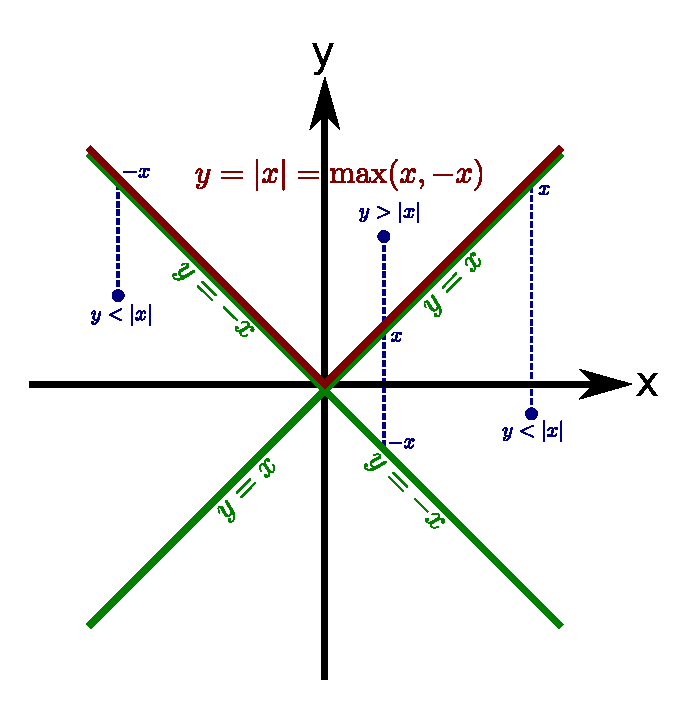
\includegraphics[width = 0.5\textwidth]{absolute_value_as_a_maximum}
}
\end{tabular}



\textbf{Example 1:}

Start with the inequality:
\[|x - 1| \leq 3\]
This inequality yields the system:
\[(x - 1 \leq 3) \wedge (-(x - 1) \leq 3)\]

Solving the first inequality, \(x - 1 \leq 3\), adding \(1\) to both sides gives:
\[x \leq 4\]
This yields the interval:
\[(-\infty, 4]\]

Solving the second inequality, \(-(x - 1) \leq 3\), multiplying both sides by \(-1\) gives:
\[x - 1 \geq -3\]
Adding \(1\) to both sides gives:
\[x \geq -2\]
This yields the interval:
\[[-2, +\infty)\]

Since both inequalities are to be satisfied, the intersection of the two intervals is to be performed:
\[(-\infty, 4] \cap [-2, +\infty) = [-2, 4]\]
The set of values of \(x\) that satisfies \(|x - 1| \leq 3\) is: 
\[[-2, 4]\]



\textbf{Example 2:}

Start with the inequality:
\[|2x - 13| > 7\]
This inequality yields the system:
\[(2x - 13 > 7) \vee (-(2x - 13) > 7)\]
(recall that the symbol \(\vee\) means ``OR")

Solving the first inequality, \(2x - 13 > 7\), adding \(13\) to both sides gives:
\[2x > 20\]
Dividing both sides by \(2\) gives:
\[x > 10\]
This yields the interval:
\[(10, +\infty)\]

Solving the second inequality, \(-(2x - 13) > 7\), multiplying both sides by \(-1\) gives:
\[2x - 13 < -7\]
Adding \(13\) to both sides gives:
\[2x < 6\]
Dividing both sides by \(2\) gives:
\[x < 3\]
This yields the interval:
\[(-\infty, 3)\]

Since only one of the inequalities needs to be satisfied, the union of the two intervals is to be performed:
\[(10, +\infty) \cup (-\infty, 3) = (-\infty, 3) \cup (10, +\infty)\]
This set of values of \(x\) that satisfies \(|2x - 13| > 7\) is:
\[(-\infty, 3) \cup (10, +\infty)\]



\textbf{Example 3:}

Start with the inequality:
\[|3x + 6| \leq x + 6\]
This inequality yields the system:
\[(3x + 6 \leq x + 6) \wedge (-(3x + 6) \leq x + 6)\]

Solving the first inequality, \(3x + 6 \leq x + 6\), subtracting \(x\) from both sides gives:
\[2x + 6 \leq 6\]
Subtracting \(6\) from both sides gives:
\[2x \leq 0\]
Dividing both sides by \(2\) gives:
\[x \leq 0\]
This yields the interval:
\[(-\infty, 0]\]

Solving the second inequality, \(-(3x + 6) \leq x + 6\), multiplying both sides by \(-1\) gives:
\[3x + 6 \geq -x - 6\]
Adding \(x\) to both sides gives:
\[4x + 6 \geq -6\]
Subtracting \(6\) from both sides gives:
\[4x \geq -12\]
Dividing both sides by \(4\) gives:
\[x \geq -3\]
This yields the interval:
\[[-3, +\infty)\]

Since both inequalities are to be satisfied, the intersection of the two intervals is to be performed:
\[(-\infty, 0] \cap [-3, +\infty) = [-3, 0]\]
This set of values of \(x\) that satisfies \(|3x + 6| \leq x + 6\) is:
\[[-3, 0]\]




\section*{Linear regression}

The relationship between two {\bf real valued} variables \(X\) and \(Y\) is often approximated by a ``line of best fit", also referred to as a ``regression line", \(Y = mX + c\). Given an arbitrary value for \(X\), the value of \(Y\) is guessed by \(Y = mX + c\). The coefficients \(m\) and \(c\) are chosen to minimize the errors that are present with the guess \(Y = mX + c\). 

To compute coefficients \(m\) and \(c\), a large number \(N\) of ``samples", also referred to as ``data points", of \((X, Y)\) value pairs are needed. Each sample needs to contain both the values of \(X\) and \(Y\), and must not be subject to ``sample bias". For the discussions to follow, the number of samples will be denoted by \(N\), and the \(i^\text{th}\) sample will be denoted by \((x_i, y_i)\), so the combined list of samples is \((x_1, y_1)\), \((x_2, y_2)\), ..., \((x_N, y_N)\).    

To aid in the discussions to follow, {\bf summation notation} will be introduced: Consider an arbitrary expression \(f(i)\) involving an integer index \(i\). Also consider lower and upper bounds for the integer index \(i\). These lower and upper bounds are denoted by the integers \(a\) and \(b\) respectively where \(a \leq b\). The sum of \(f(i)\) where \(i\) ranges from \(a\) to \(b\) is denoted by:
\[\sum_{i=a}^b f(i) = f(a) + f(a+1) + f(a+2) + \cdots + f(b)\] 

The total error \(\epsilon\) that it is to be minimized is the following:
\[\epsilon = \sum_{i=1}^N ((mx_i + c) - y_i)^2 = ((mx_1 + c) - y_1)^2 + ((mx_2 + c) - y_2)^2 + \cdots + ((mx_N + c) - y_N)^2\]
For each \(i = 1, 2, ..., N\), consider the \(i^\text{th}\) sample \((x_i, y_i)\). \(mx_i + c\) is the predicted value of \(Y\), while \(y_i\) is the true value of \(Y\). The difference between the prediction and the true value is \((mx_i + c) - y_i\), and squaring this difference gives a \emph{positive} value \(((mx_i + c) - y_i)^2\), which quantifies the error present in the \(i^\text{th}\) sample. The sum of these errors is the total error \(\epsilon\).

The first step in computing the coefficients \(m\) and \(c\) is to compute the ``center of mass" of all of the data points. The center of mass, denoted by \((E_X, E_Y)\) is the average \(X\) value, and the average \(Y\) value:
\[(E_X, E_Y) = \left(\frac{1}{N}\sum_{i=1}^N x_i, \frac{1}{N}\sum_{i=1}^N y_i\right) = \left(\frac{x_1 + x_2 + \cdots + x_N}{N}, \frac{y_1 + y_2 + \cdots + y_N}{N}\right)\] 

The regression line will {\bf always} pass through the center of mass \((E_X, E_Y)\), so all that remains is to compute the gradient \(m\).

To compute \(m\), 3 more quantities need to be defined and computed. The variance of \(X\), denoted by \(V_X\); the variance of \(Y\), denoted by \(V_Y\); and the covariance of \(X\) and \(Y\), denoted by \(C_{XY}\).

The variances \(V_X\) and \(V_Y\) are measures of the spread of the \(X\) and \(Y\) sample values respectively:
\[V_X = \frac{1}{N}\sum_{i=1}^N (x_i - E_X)^2 = \frac{(x_1 - E_X)^2 + (x_2 - E_X)^2 + \cdots + (x_N - E_X)^2}{N}\]
\[V_Y = \frac{1}{N}\sum_{i=1}^N (y_i - E_Y)^2 = \frac{(y_1 - E_Y)^2 + (y_2 - E_Y)^2 + \cdots + (y_N - E_Y)^2}{N}\]

The covariance \(C_{XY}\) is:
\begin{align*}
C_{XY} = & \frac{1}{N}\sum_{i=1}^N (x_i - E_X)(y_i - E_Y) \\
= & \frac{(x_1 - E_X)(y_1 - E_Y) + (x_2 - E_X)(y_2 - E_Y) + \cdots + (x_N - E_X)(y_N - E_Y)}{N}
\end{align*}

With \(V_X\), \(V_Y\), and \(C_{XY}\) known, the slope \(m\) is:
\[m = \frac{C_{XY}}{V_X}\]

The regression line passes through the center of mass \((E_X, E_Y)\), and has a slope of \(m\), so the regression line has the equation:
\[Y - E_Y = m(X - E_X) \iff Y = E_Y + (mX - mE_X) \iff Y = mX + (E_Y - mE_X)\]  

Lastly, it should be noted that the regression line \(Y = mX + c\) only guesses at \(Y\), and will rarely, if ever, be perfectly accurate. A means of quantifying the accuracy of the regression line is the correlation coefficient \(r\):
\[r = \frac{C_{XY}}{\sqrt{V_X V_Y}}\] 

By mathematical necessity, the correlation coefficient \(r\) is confined to the interval \([-1, 1]\). It is important to note that the actual slope of the regression line has no impact on the value of \(r\), with the sole exception being the slope's sign. The value of \(r\) has the following interpretations: \\
\begin{tabular}{cc}
\parbox{0.5\textwidth}{
\begin{itemize}
\item If \(r = 1\), then the sample points make a perfect line with an increasing slope. 
\item If \(0 < r < 1\), then the sample points form a cloud that surrounds the regression line with an increasing slope. 
\item If \(r = 0\), then the two variables are independent of each other, and the slope of the regression line is \(0\). When this happens, there is no correlation between \(X\) and \(Y\). 
\item If \(-1 < r < 0\), then the sample points form a cloud that surrounds the regression line with a decreasing slope. 
\item If \(r = -1\), then the sample points make a perfect line with a decreasing slope. 
\end{itemize}
} & \parbox{0.5\textwidth}{
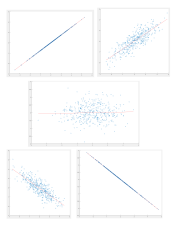
\includegraphics[width = 0.5\textwidth]{correlation_coefficient_scenarios}
}
\end{tabular} \\
The correlation coefficient \(r\) quantifies the accuracy of the regression line with values of \(r\) that are further from \(0\) corresponding to better accuracy. Perfect accuracy occurs when \(r = \pm 1\), and no accuracy occurs when \(r = 0\).

In summary, the complete process of finding the regression line \(Y = mX + c\) and the correlation coefficient \(r\) is 
\begin{itemize}
\item Compute \(E_X = \frac{1}{N}\sum_{i=1}^N x_i = \frac{x_1 + x_2 + \cdots + x_N}{N}\) 
\item Compute \(E_Y = \frac{1}{N}\sum_{i=1}^N y_i = \frac{y_1 + y_2 + \cdots + y_N}{N}\) 
\item Compute \(V_X = \frac{1}{N}\sum_{i=1}^N (x_i - E_X)^2 = \frac{(x_1 - E_X)^2 + (x_2 - E_X)^2 + \cdots + (x_N - E_X)^2}{N}\) 
\item Compute \(V_Y = \frac{1}{N}\sum_{i=1}^N (y_i - E_Y)^2 = \frac{(y_1 - E_Y)^2 + (y_2 - E_Y)^2 + \cdots + (y_N - E_Y)^2}{N}\) 
\item Compute \(C_{XY} = \frac{1}{N}\sum_{i=1}^N (x_i - E_X)(y_i - E_Y) = \frac{(x_1 - E_X)(y_1 - E_Y) + (x_2 - E_X)(y_2 - E_Y) + \cdots + (x_N - E_X)(y_N - E_Y)}{N}\) 
\item Compute \(m = C_{XY}/V_X\) 
\item Compute \(c = E_Y - mE_X\) 
\item Compute \(r = C_{XY}/\sqrt{V_X V_Y}\)
\end{itemize}

In the image below, an example regression line is computed using Microsoft Excel.

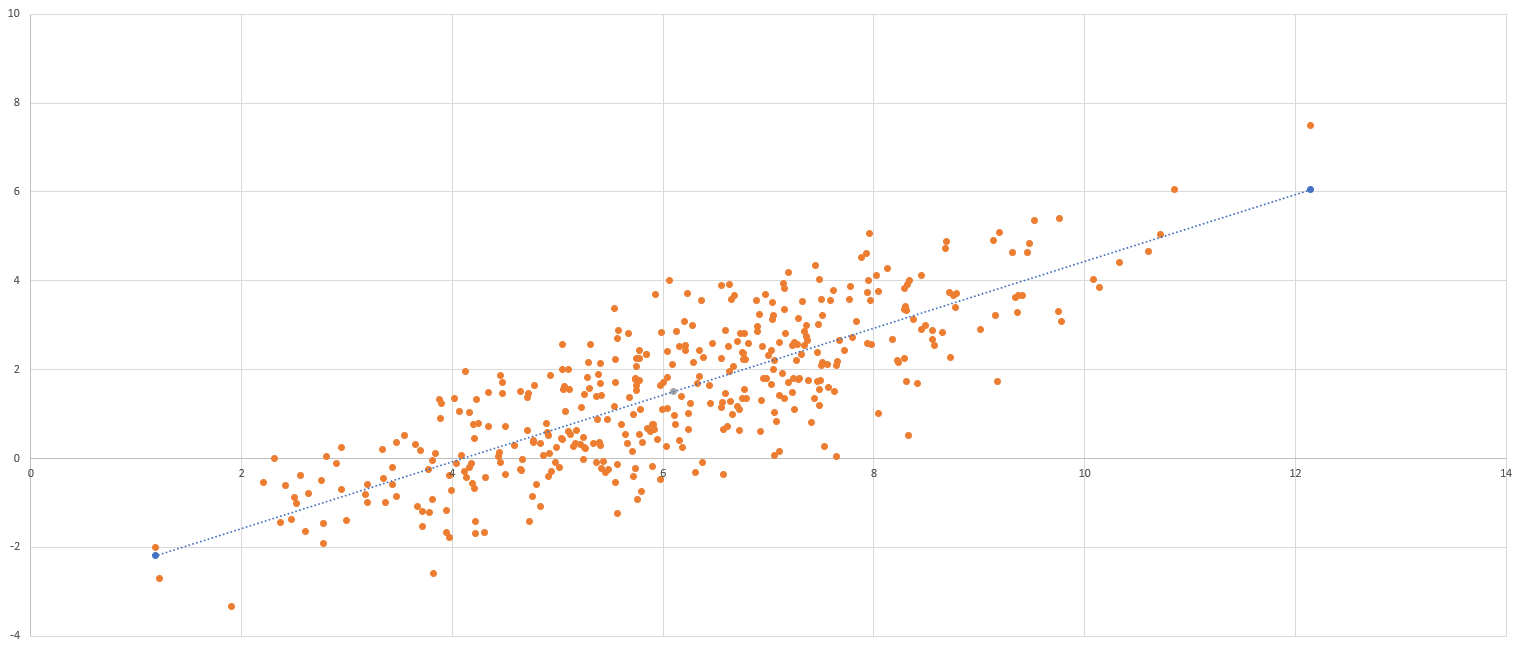
\includegraphics[width = \textwidth]{Linear_regression_example}


%\subsection*{Proofs}





\end{document}












